\section{Nondeterministiske automater}
\begin{frame}
\frametitle{Ækvivalens ml. Regulære udtryk og FA'er}
  \begin{itemize}[<+->]
  \item Definition af NFA’er og deres sprog
\item Delmængdekonstruktionen:  NFA $\rightarrow$ FA
\item Definition af NFA-$\Lambda$’er og deres sprog
\item $\Lambda$-eliminering:  NFA-$\Lambda$ $\rightarrow$ FA
\item Kleenes sætning: regulært udtryk $\rightarrow$ NFA-$\Lambda$ $\rightarrow$ NFA $\rightarrow$ FA $\rightarrow$ regulært udtryk
  \end{itemize}
\end{frame}


\begin{frame}
\frametitle{Nondeterministiske automater}
\begin{itemize}[<+->]
\item  NFA’er: som FA’er men
\item Der er ikke altid præcis én udgående transition pr. alfabetsymbol for hver tilstand
\item Automaten accepterer en streng, hvis det er muligt at ``gætte'' en vej til accept
\end{itemize}

\end{frame}

\begin{frame}
\frametitle{Eksempel}

\begin{columns}
  \begin{column}{9cm}
    \begin{itemize}[<+->]
    \item Hvordan laver man en automat, der svarer til det regulære
      udtryk $(11 + 110)^*0$ ?

    \item Det er ikke trivielt med FA’er...

    \item En nondeterministisk automat:
    \end{itemize}
  \end{column}
\pause
  \begin{column}{5cm}
      \includegraphics[scale=0.4]{images/2_seminar_nondet}
  \end{column}
\end{columns}
\end{frame}
\begin{frame}
\frametitle{Formel definition af NFA}
En nondeterministisk endelig automat (NFA) er et 5-tupel $(Q, \Sigma, q_0, A, \delta)$ hvor
 
\begin{itemize}[<+->]
\item $Q$ er en endelig mængde af tilstande
\item $\Sigma$ er et alfabet
\item $q_0\in Q$ er en starttilstand
\item $A\subseteq Q$ er accepttilstande
\item $\delta$: $Q\times \Sigma \rightarrow$ \alert{$2^Q$} er en transitionsfunktion\\
  Det betyder at $\delta(q,a)$ giver en \emph{mængde} af tilstande.
\end{itemize}
\end{frame}
\begin{frame}
\frametitle{Eksempel på en NFA}
\begin{columns}
\column{9cm}Her er den grafiske representation af en automat:
\column{3cm}\includegraphics[scale=0.3]{images/2_seminar_nondet_states}
\end{columns}
\begin{itemize}[<+->]
  \item Den representerer 5-tuplet:
  \item $Q=\{q_0,q_1,q_2,q_3,q_4\}$
  \item $\Sigma = \{0,1\}$
  \item $A=\{q_4\}$
  \item
      $\delta$ : $Q\times \Sigma \rightarrow 2^Q$ Er funktionen i
      denne tabel: \scalebox{0.7}{
        \begin{tabular}{|l|ll|}
          \hline
          & 0 & 1 \\
          \hline
          $q_0$ & $\{q_4\}$ & $\{q_1, q_2\}$ \\
          \hline
          $q_1$ & $\emptyset$ & $\{q_0\}$ \\
          \hline
          $q_2$ & $\emptyset$ & $\{q_3\}$ \\
          \hline
          $q_3$ & $\{q_0\}$ & $\emptyset$ \\
          \hline
          $q_4$ & $\emptyset$ & $\emptyset$ \\
          \hline
        \end{tabular}}

  \end{itemize}
\end{frame}
\begin{frame}
\frametitle{Sproget af en NFA}
Givet en NFA $M=(Q, \Sigma, q_0, A, \delta)$:
\begin{itemize}[<+->]
\item Definer den udvidede transitionsfunktion:
\[\delta^*(q, x) = \begin{cases}
  \{q\} & \text{ hvis } x=\Lambda \\
  \bigcup_{r\in \delta^*(q,y)}\delta(r, a)& \text{ hvis } x=y\cdot a
\end{cases}
\]
\item $x\in \Sigma^*$ accepteres af en NFA $M$ hvis og kun hvis $\delta^*(q_0,x) \cap A \neq \emptyset$
\item $L(M)=\{x | x \text{ accepteres af } M\}$
\end{itemize}
\end{frame}
\begin{frame}
\frametitle{NFA'er er ofte mindre end FA'er}
\begin{itemize}[<+->]
\item $L_{42}=\{x \mid |x|\geq 42 \wedge \text{ 42 tegn fra højre er et 1} \}$
\item Sidste seminar viste vi at det kræver mindst $2^{42}$ tilstande
  at lave en FA der genkender $L_{42}$
\item En \alert{N}FA der genkender $L_{42}$ med 43 tilstande:
\includegraphics[scale=0.4]{images/2_seminar_L42_NFA}
\end{itemize}
\end{frame}
\begin{frame}
\frametitle{Quiz}
\begin{columns}
\column{5cm} Bliver strengen 110110 accepteret af denne automat?
\column{5cm}
\includegraphics[scale=0.4]{images/2_seminar_quiz_NFA}
\end{columns}
\pause
Ja! der findes en sti til accept:
\[
q_0 \rightarrow q_2 \rightarrow q_3 \rightarrow q_0 \rightarrow q_1 \rightarrow q_0 \rightarrow q_4
\]
\pause
Vi kan systematisk lede efter sådan en sti:
$\{q_0\} \pause \rightarrow \{q_1, q_2\} \pause \rightarrow 
\{q_0, q_3\} \pause \rightarrow $\\
$\{q_4, q_0\} \rightarrow \{q_1, q_2\} \rightarrow \{q_0, q_3\} \rightarrow 
\{q_4, q_0\} 
$
\end{frame}
\begin{frame}
\frametitle{Øvelser:}
\begin{itemize}
\item [Martin]: opg. 4.2. (p. 156)

Drawing an NFA and using the definition of $\delta^*$
\end{itemize}
\end{frame}

\section{Determinisering}
\begin{frame}
\frametitle{Enhver FA kan oversættes til en NFA}
\begin{itemize}[<+->]
\item Hvis man ser på den grafiske repræsentation, så er det trivielt,
  en FA er bare en simpel NFA.
\item Formelt: givet en FA: $N=(Q, \Sigma, q_0, A, \delta)$
\item Konstruer en NFA: $M=(Q, \Sigma, q_0, A, \delta')$ hvor:
  
\[\delta'(q,a) = \{\delta(q,a)\}\]
\item Husk bevis for korrekthed! $L(M)=L(N)$ fordi... (induktion i længden af en inputstreng)
\end{itemize}
\end{frame}

\begin{frame}
\frametitle{Enhver NFA kan oversættes til en FA}
\begin{center}
  \includegraphics[scale=0.4]{images/2_seminar_convert}
\end{center}
\pause

Dette kaldes determinisering
\end{frame}

\begin{frame}
\frametitle{Delmængdekonstruktionen (determinisering)}
Givet en NFA: $N=(Q, \Sigma, q_0, A, \delta)$

Konstruer en FA: $M=(Q', \Sigma, q_0', A', \delta')$
\pause
\begin{itemize}[<+->]
\item $Q'=\alert{2^{Q}}$ (tilstandene i FA'en svarer til en mængde af tilstande i NFA'en)
\item $q_0' = \{q_0\}$
\item $A' = \{q \in Q' | A \cap q \neq \emptyset \}$
\item $\delta'(q, a) = \bigcup_{r\in q}\delta(r,a)$
\item Husk bevis for korrekthed...
\end{itemize}
\end{frame}
\begin{frame}
  \frametitle{Bevis for korrekthed af delmængdekonstruktionen}
\begin{itemize}[<+->]
\item Husk definitionen for $L(M)$ og $L(N)$
\[L(M) = \{x | \delta'^*(q_0', x) \in A'\]
\[L(N) = \{x | \delta^*(q_0, x) \cap A \neq \emptyset\]
\item Lemma:
\[\forall x\in \Sigma^*: \delta'^*(q_0', x) = \delta^*(q_0, x)\]
Bevis: induktion i strukturen af $x$...
\item $ \delta'^*(q_0', x) \in A' \overset{\text{\tiny{lemma}}}{\Leftrightarrow} 
delta^*(q_0, x) \in A' \overset{\text{\tiny{def af A}}}{\Leftrightarrow} \delta^*(q_0, x) \cap A \neq \emptyset$
\item D.v.s. $L(M)=L(N)$
\end{itemize}
\end{frame}

\begin{frame}
\frametitle{Nøjes med opnåelige tilstande}
\begin{itemize}[<+->]
\item Delmængdekonstruktionen bruger $Q' = 2^Q$
\item Som ved produktkonstruktionen: I praksis er hele tilstandsrummet
  sjældent nødvendigt
\item Som sidste gang: Kun tilstande, der er opnåelige fra
  starttilstanden er relevante for sproget (Bevis dette: Opg. 3.29, p. 117)
\end{itemize}
\end{frame}
\begin{frame}
\frametitle{Øvelser}
\begin{itemize}
\item [Martin] Opg. 4.10 (a+e) (p. 157)\\
Udfør selv delmængdekonstruktionen.
\end{itemize}
\end{frame}